Additional tools are being developed for the regional simulations. These applications are needed to create the knowledge bases used for the built environment in the regional simulations. While not complicated in design, these applications are useful for NHERI researchers to gather additional information. This chapter contains up to a level 3 description of the software.

\section{Level 1: Context for Data Gathering Backend Applications}

A level 1 description showing the context of the software provided for data gathering is shown in \Cref{fig:contextData}. It shows that the software uses information available on the WWW to build the datasets.

 \begin{figure}[!htbp]
  \centering {
    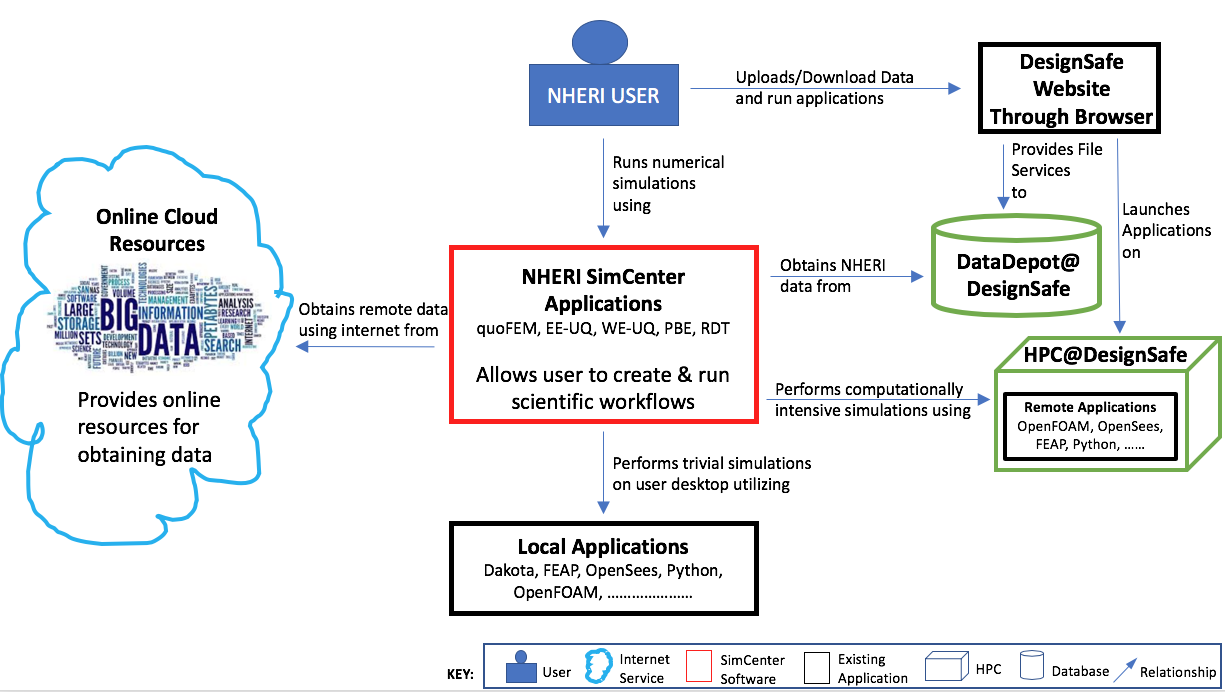
\includegraphics[width=0.95\textwidth]
    {images/context.png} }
  \caption{System Context Diagram for Data Gathering Applications}
  \label{fig:contextData}
\end{figure}

\section{Level 2: Container Diagram for Data Gathering Applications}
A level 2 container diagram shows that this software is again broken into 2; initial software to ascertain parcel level building information and then software to collect additional data.

\begin{figure}[!htbp]
  \centering {
    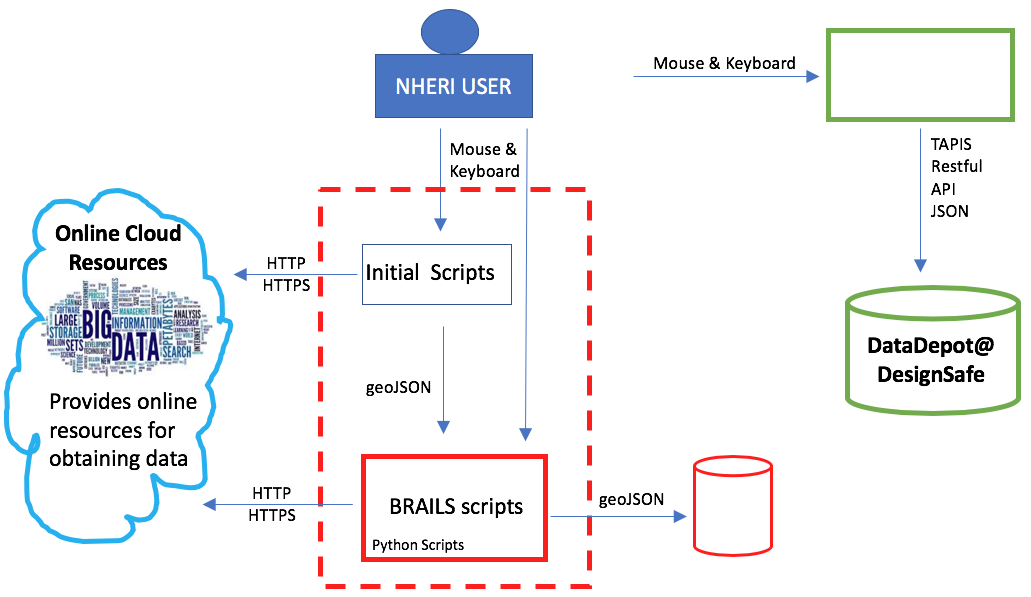
\includegraphics[width=0.95\textwidth]
    {images/containerData.png} }
  \caption{System Container Diagram for Data Gathering Applications}
  \label{fig:containerData}
\end{figure}

 
\section{Level 3: Component Diagram for BRAILS container}

A number of applications are provided, some of which utilize Selenium to scrape assessors’ databases for information at the parcel level on building data. Some applications utilize Machine learning to ascertain building properties, e.g. roof shapes and first floor levels. These applications, and trained neural networks are included in the BRAILS framework. The applications cannot ascertain all the information for the regional datasets. Where information is missing SURF.ET-AI.py is used. SURF.ET-AI.py is part of SURF package. SURF is used to fill in the missing data.
 
\begin{figure}[!htbp]
  \centering {
    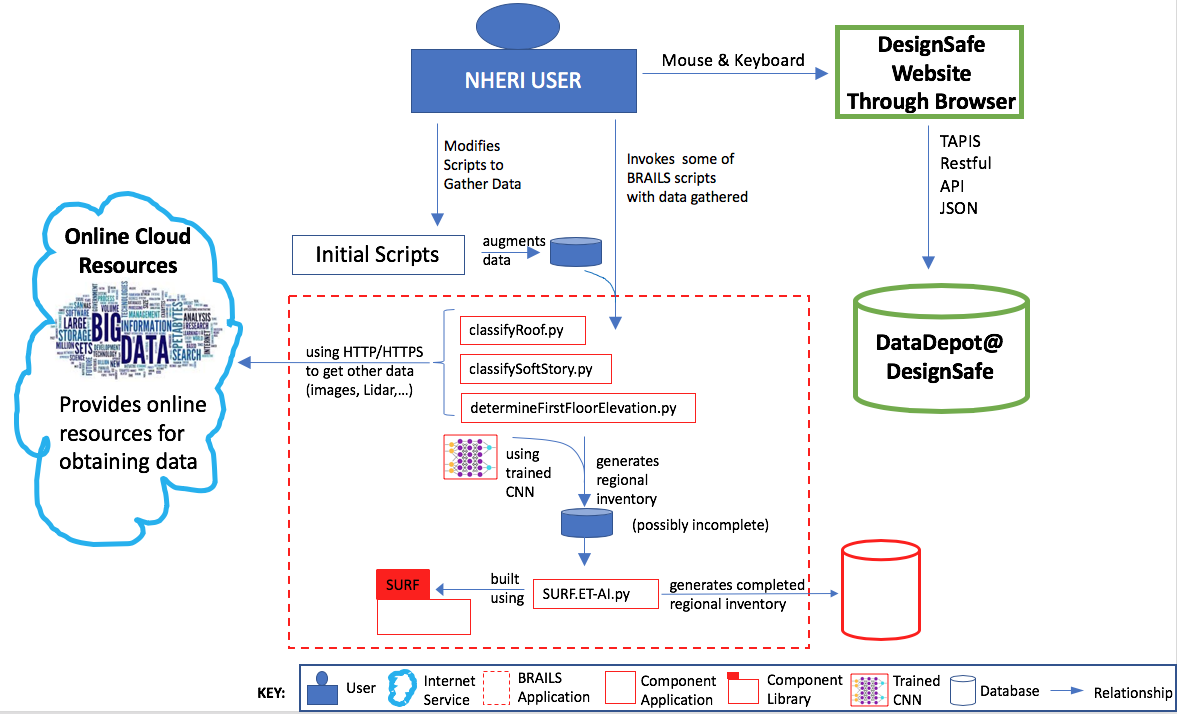
\includegraphics[width=0.95\textwidth]
    {images/componentBRAILS.png} }
  \caption{Component Diagram for BRAILS}
  \label{fig:componentBRAILS}
\end{figure}
